\section{Introduction}
%\textbf{Power is an instantaneous quantity, and cannot be consumed or saved, *energy* can be.}
% **** MOVING BELOW TEXT TO ABSTRACT ****
%Monitoring and reducing the energy consumption of servers in data centers is critical.
%The importance of this task is magnified by the presence of increasingly constrained energy budgets in data centers~\cite{SmoothOperator, Dynamo}.
%Reducing the power drawn by 10,000 datacenter servers by 10 watts (10 joules/second) would result in energy savings that could power approximately 100 US households with a corresponding financial saving of \$100,000/year\footnote{\textbf{(provide details of calculation)}}.
%TODO MISSING NUMBER IN FOOTNOTE

% **** MOVING BELOW TEXT TO ABSTRACT ****
%The factors that affect a server's energy use arise from the complex interactions between the application workload,  software stack, and the hardware characteristics and configuration of the node itself.
%This paper sheds light on %concerns
%the task of tuning hardware parameters to control the time and energy required for IO sensitive, system-centric workloads typical of cloud services.  We reveal the significant impact that static tuning can have and the influence of operating systems software on the performance of the aforementioned applications.  Figure~\ref{fig:setup} illustrates our experimental overview of this tuning task.
%We discuss our experimental procedure in more detail in section~\cref{sec:overview}.
%We are particular interested in exposing the impact that the operating system (OS) software structure has on this task.  

%fix role and fix software,
The hardware nodes of a cloud service provider are often dedicated to running a single cloud service component.
One hopes that this dedicated nature (i.e. fixed role in the service using a fixed software stack) can be exploited to obtain the required performance while minimizing the energy used (and thus the cost for providing the service). The importance of this task is magnified by the presence of increasingly constrained energy budgets in data centers~\cite{SmoothOperator, Dynamo}. General purpose operating systems (OSes) such as Linux, have been designed and implemented to support a broad range of user software as well as the concurrent execution of competing applications. Thus, they have evolved to include support for dynamically adjusting various hardware settings. Dedicating a node to a single application suggests that one may be able to manually tune the node's hardware parameters to fixed values and obtain higher efficiency than allowing the OS to dynamically adjust them.  Furthermore, it is possible that the impact of hardware tuning can be magnified if one starts with an application specific OS that has been designed and implemented for running a single dedicated application.  Researchers have proposed  such systems, referred to as library OSes~\cite{ebbrt,ix,arrakis, exokernel} or unikernels~\cite{rumpkernel, unikernels, aliraza}.  

\begin{figure}
  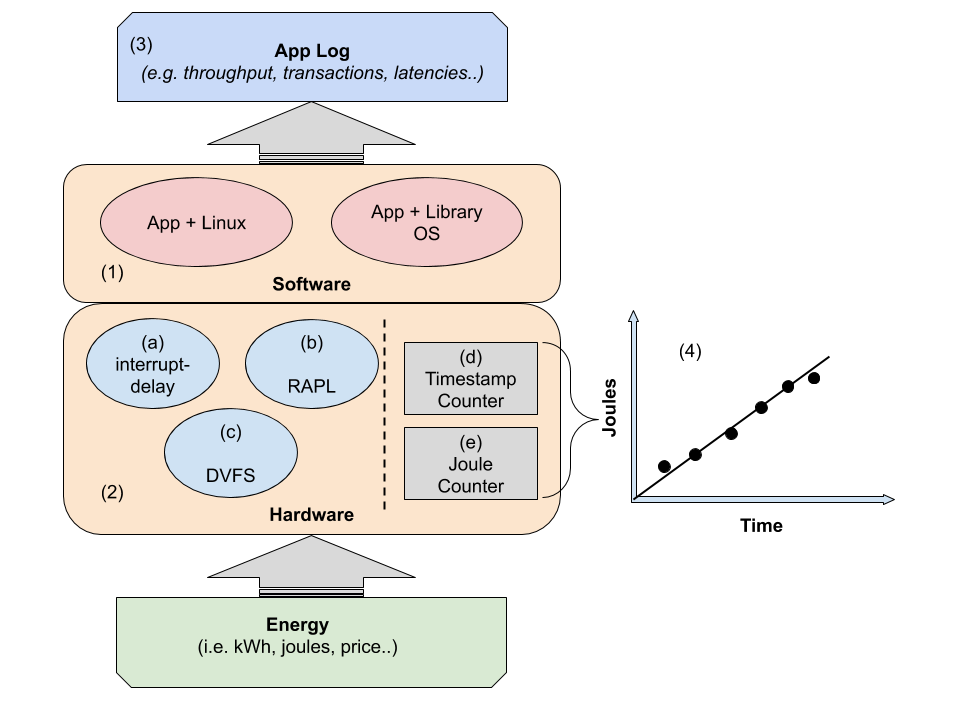
\includegraphics[width=8.5cm]{figures/setup.png}
  \caption{ Overview of Energy Tuning Task:  1) Configure a hardware node with  one of two OS-Application software stacks (Linux or library OS)
  2) Set a specific value for each of the three hardware parameters being tuned: a) NIC interrupt-delay,  b) RAPL, and c) processor DVFS. Now run an application-specific benchmark which introduces load on the hardware node.
  3) During the execution of the benchmark, collect log data using the processor's performance monitoring counters (PMCs) as well as d) the time at which a NIC interrupt occurs and e) the number of Joules consumed at that point.  Also gather an application-specific metric related to the quality of the application's performance (e.g. throughput, latency, etc. 4) Using the recorded logs and performance data, identify settings for each OS that minimize the Energy Delay Product (EDP) required to do a fixed amount of application work. Ideally, for one application workload, one OS stack will clearly yield better values for both time and energy.  If, on the other hand, the interactions within the OSes are more subtle than that, their performance will reflect a more subtle trade-off in time versus energy.}
 \label{fig:setup}
\end{figure}

This paper presents the results of manually tuning three hardware parameters across three network applications and on two distinct OSes.
Figure~\ref{fig:setup} illustrates our experimental overview of this tuning task.
We discuss our experimental procedure in more detail in section~\ref{sec:overview}.
Section~\ref{sec:knobs} discusses the hardware parameters which we tune. The two operating systems we evaluate with respect to static tuning are Linux and a specialized application specific library OS\footnote{(anonymized for submission)} written in C++.   We compare our results to Linux configured to its default behaviour: where two hardware parameters are dynamically tuned using built-in algorithms while the third has a default fixed value.   



%Two of the hardware features have exist on modern processors and been applied in the past towards saving energy, they are commonly referred to as Running Average Power Limit (RAPL)~\cite{intel_rapl, 10.1145/2678373.2665718, 10.1145/3177754, zhang2015quantitative} and Dynamic Voltage Frequency Scaling (DVFS)~\cite{10.1145/2024723.2000103, 10.1145/2806777.2806848, rubik, 10.1145/.3303981} methods. We introduce a third hardware feature exposed by the network interface card (NIC), packet receive interrupt-delay, which lies directly on the packet processing path. To lend credence to this third parameter, we found that out of the over 5000 potential adjustable registers in the the NIC~\cite{82599} used in our experiments, the interrupt-delay value was the only one where a dynamic policy in Linux for tuning it exists. 

To evaluate and compare the effectiveness of tuning the three hardware parameters across the OS configurations, we adapt the energy delay product (EDP) metric from the architecture community~\cite{Gonzalez1996EnergyDI}.
%YA:compaction
We use a workload-specific measure (e.g. number of message round-trips or web requests) to define work done on the computational nodes and define delay as the time taken to do this work and energy as the joules consumed in the process. The value of EDP on each system - the energy used multiplied by the delay - becomes an indicator of energy efficiency. EDP is a useful metric as it reflects both the time and energy spent to accomplish some application work;  ideally, one can find an OS and hardware parameter setting that reduces both.
%Rather than defining the work done in terms of instructions, we use a workload-specific measure, such as the number of message round trips or web requests. For a particular application scenario, we define delay as the time taken to accomplish this work and energy as the joules consumed in the process.  The measure of energy delay product (EDP) on each system then becomes an indicator of energy efficiency. EDP is a useful metric as it reflects both the time and energy spent to accomplish some application work;  ideally, one can find an OS and hardware parameter setting regime that reduces both.


%There are three \textit{systems} that we compare EDP across the four applications: 1) Linux default where the dynamic policy for adjusting the hardware parameters are still enabled, 2) Linux tuned where the dynamic policy is disabled and per-application static values for the hardware parameters are used instead, and 3) library OS tuned in similar manner to Linux tuned.

%These results are then compared to baseline results obtained using Linux with its default dynamic behavior for adjusting the settings. 

%To demonstrate the intricacies and interplay between hardware parameter tuning across different applications and systems software, we modify the network device driver of both Linux and EbbRT to gather detailed per packet information along with other various hardware counters and energy data (see section~\cref{sec:log_collect}) on every network interrupt for the life time each application experimental run. This fine-grained data not only reveals the aggregate time and energy trade-off a particular software and hardware configuration, it also provides insight into the instantaneous behaviour that the OS has on and between every network interaction. Methodologically, we exhaustively gather a large data set which documents the behaviour of the systems across all the applications across a sweep of the three hardware parameters.

Experimentally, we find that in our three workloads one can reduce the EDP by using tuned fixed hardware parameters rather than the default Linux dynamic behaviour. Furthermore, the library OS can be tuned to achieve an even greater EDP reduction.
As an example, consider the energy and time required for running a memcached~\cite{memcached} server to satisfy five million requests at a rate of 600K queries per-second while maintaining a 99\% tail latency below a  500{$\mu$}s service level agreement (SLA).
Using default Linux, we measured total energy use on the processor at {\textasciitilde}1050 joules for {\textasciitilde}8.5 seconds (EDP = 8925 joules x second) with a 99\% tail latency of 134.4{$\mu$}s. Searching through the static settings, we find fixed hardware parameter values for Linux that save a significant {\textasciitilde}440 joules ({\textasciitilde}42\%) with a tail latency of 475{$\mu$}s.  Tuning the parameters when using the library OS yields an even greater savings of {\textasciitilde}635 joules ({\textasciitilde}60\%) with a tail latency 105{$\mu$}s. These dramatic savings indicate that OS structure matters when it comes to energy efficiency, even for running IO workloads with significant idle time. Further, these results suggest that global data-center energy consumption could significantly benefit from improving operating system support for executing a single fixed and dedicated applications. 

%Tuning Linux with fix parameters, such that the EDP is minimized results in a consumption of {\textasciitilde}700 Joules and {\textasciitilde}8.5 seconds (EDP=15291.5 JouleSeconds with a 99\% tail latency of 475.2{$\mu$}s).  However, tuning the parameters when using EbbRT, results in a consumption of {\textasciitilde}425 Joules and {\textasciitilde}8.5 seconds (EDP=3612.5 JouleSeconds with a 99\% tail latency of 365.8{$\mu$}s).  Tuning with respect to EDP in this case is the same as minimizing energy given that EDP is minimized, for both Linux and EbbRT, at {\textasciitilde}8.5 seconds. 

The contributions of this paper are as follows: 1) A new methodology for the detailed study of energy consumption that includes the interaction of systems software, 2) an adaption and application of EDP to the study of complex IO intensive software stacks, 3) a quantification of the impact of jointly tuning network interrupt delay, DVFS, and RAPL on Linux's energy consumption compared to its default dynamic policies, 4) exposure of the dramatic benefits of statically tuning hardware parameters for dedicated workloads on Linux, and 5) a novel quantification of the benefits on energy consumption of using a baremetal application-specific library OS.


The rest of the paper is presented in the following way: Section\ref{sec:overview} discusses energy optimization, defining EDP (the core metric used), the three hardware parameters that we tune, and our general experimental methodology and infrastructure. Section\ref{sec:apps} presents our three workloads and core results for each.  Specifically, we begin with a study of a simple network scenario in which two systems are configured to exchange a single stream of packets of a fixed size.  We then describe our study of a NodeJS webserver driven by a single stream of sequential request over a persistent connection.  Moving up in complexity, we present results from our multicore memcached study under a stringent SLA objective. 
%Finally, we present results from exercising a server running the Silo in-memory database combined with memcached. We conclude with a brief summary and discussion of our future work.  